\documentclass[crop,border={2pt 2pt 2pt 2pt},tikz]{standalone}
\usepackage{braket}
\usepackage{bbold}
\usepackage{bm}
\usepackage{amsmath}
\usepackage{tikz-3dplot}
% \usepackage{physics}

\usetikzlibrary{backgrounds,decorations.markings, calc}
\tikzset{>=latex}
\tikzset{->-/.style={decoration={
  markings,
  mark=at position .55 with {\arrow{>}}},postaction={decorate}}}
\begin{document}
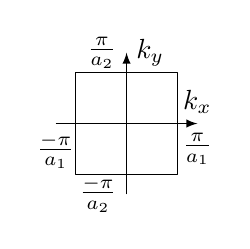
\begin{tikzpicture}[line join = round]
    \draw[] (-0.65,-0.65) rectangle (0.65,0.65);
    \draw[->] (-0.9,0) node[anchor=north] {$\frac{-\pi}{a_1}$} -- (0.9,0) node[anchor = south] {$k_x$} node[anchor = north] {$\frac{\pi}{a_1}$};
    \draw[->] (0,-0.9) node[anchor= east] {$\frac{-\pi}{a_2}$} -- (0,0.9) node[anchor = west] {$k_y$} node[anchor = east] {$\frac{\pi}{a_2}$};  
\end{tikzpicture}
\end{document}